\documentclass{article}
\usepackage{amsmath, sfmath, multicol, tkz-euclide, array, enumerate, tcolorbox, tabularray}
\renewcommand{\familydefault}{\sfdefault}
\setlength{\parindent}{0cm}
\pagestyle{empty}
\usepackage[left=1in, top=0.5in, right=1in, bottom=0.5in]{geometry}
\tikzset{>=stealth, label style/.append style={font=\footnotesize}}
\tcbset{colback=white}

\newcounter{example}[section]
\newenvironment{example}[1][]{\refstepcounter{example}\par\medskip
   {\color{red}\textbf{Example~\theexample. #1}}}{\medskip}

\begin{document}

\section*{Polygon Angle-Sum Theorems}

\begin{tcolorbox}[colframe=orange!70!white, coltitle=black, title=\textbf{Today I Can}]
\begin{enumerate}
    \item Find the interior angles and sums of interior angles of polygons.
    \item Find the exterior angles and sums of exterior angles of polygons.
\end{enumerate}
\end{tcolorbox}
\bigskip 

\begin{tabular}{p{0.2\textwidth}p{0.2\textwidth}p{0.2\textwidth}p{0.2\textwidth}}
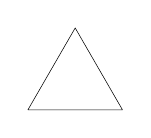
\begin{tikzpicture}[scale=0.6]
\tkzDefPoints{0/0/A, 2/0/B}
\tkzDefShiftPoint[A](60:2){C}
\tkzDrawPolygon(A,B,C)
\end{tikzpicture}
&
\begin{tikzpicture}[scale=0.6]
\tkzDefPoints{0/0/A, 2/0/B, 2/2/C, 0/2/D}
\tkzDrawPolygon(A,B,C,D)
\end{tikzpicture}
&
\begin{tikzpicture}[scale=0.6]
\tkzDefPoints{0/0/A, 2/0/B}
\tkzDefShiftPoint[B](72:2){C}
\tkzDefShiftPoint[A](108:2){E}
\tkzDefShiftPoint[E](36:2){D}
\tkzDrawPolygon(A,B,C,D,E)
\end{tikzpicture}
&
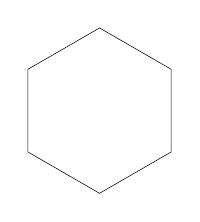
\begin{tikzpicture}[scale=0.6]
\tkzDefPoints{0/0/O}
%\tkzDrawCircle[R](O,1.75cm)
\tkzDefShiftPoint[O](90:1.75cm){A}
\tkzDefShiftPoint[O](150:1.75cm){B}
\tkzDefShiftPoint[O](210:1.75cm){C}
\tkzDefShiftPoint[O](270:1.75cm){D}
\tkzDefShiftPoint[O](330:1.75cm){E}
\tkzDefShiftPoint[O](30:1.75cm){F}
\tkzDrawPolygon(A,B,C,D,E,F)
\end{tikzpicture}
\end{tabular}
\bigskip 

\begin{center}
\setlength{\extrarowheight}{5pt}
\begin{tabular}{|c|c|c|c|}
\hline
\textbf{Polygon}    &   \textbf{\# of Sides}    &   \textbf{\# of Triangles Formed} &   \textbf{Interior Angle Sum}  \\[5pt] \hline
Triangle    &   3   &   1   &   1(180) = 180    \\[5pt] \hline
Quadrilateral   &   4   &   2   &   2(180) = 360    \\[5pt]    \hline
Pentagon    &   5   &   3   &   3(180) = 540    \\[5pt] \hline
Hexagon &   6   &   4   &   4(180) = 720    \\[5pt] \hline
$n$-gon &   $n$ &   &   \\[5pt] \hline
\end{tabular}
\end{center}
\bigskip 

\begin{tcolorbox}[colframe=black!20!white, opacitybacktitle=0.1, coltitle=black, title=\textbf{Polygon Angle-Sum Theorem}]
The sum of the measures of the interior angles of an $n$-gon is 
\vspace{18pt}
\end{tcolorbox}

\begin{example}
What is the sum of the interior angles of each of the following?

\begin{enumerate}[(a)]
\begin{multicols}{2}
    \item Heptagon (7 sides)
    \item 17-gon
\end{multicols}
\vspace{0.25in}
    \item The sum of the interior angle measures of a polygon is 1980. How many sides does it have?
\end{enumerate}
\end{example}

\vspace{0.6in}

\begin{example}
Find the measure of the indicated angle in each figure.
\begin{multicols}{2}
\begin{enumerate}[(a)]
    \item What is $m\angle Y$ in pentagon $TODAY$?
    \item What is $m\angle G$ in quadrilateral $EFGH$?
\end{enumerate}
\end{multicols}
\begin{minipage}{0.5\textwidth}
    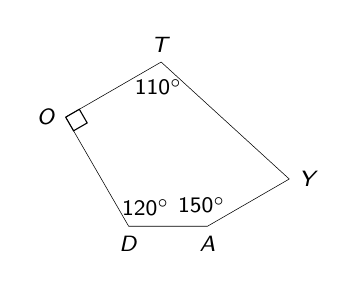
\begin{tikzpicture}[scale=0.8]
    \tkzDefPoints{0/0/D, 1.25/0/A}
    \tkzDefShiftPoint[A](30:1.5){Y}
    \tkzDefShiftPoint[D](120:2){O}
    \tkzDefShiftPoint[O](30:1.75){T}
    \tkzDrawPolygon(T,O,D,A,Y)
    \tkzLabelPoints[below](D,A)
    \tkzLabelPoints[left](O)
    \tkzLabelPoints[above](T)   
    \tkzLabelPoints[right](Y)
    \tkzMarkRightAngle(D,O,T)
    \tkzLabelAngle[pos=0.35,xshift=0.03in](A,D,O){\footnotesize $120^\circ$}
    \tkzLabelAngle[pos=0.35](Y,A,D){\footnotesize $150^\circ$}
    \tkzLabelAngle[pos=0.4](O,T,Y){\footnotesize $110^\circ$}
    \end{tikzpicture}
\end{minipage}
\begin{minipage}{0.4\textwidth}
    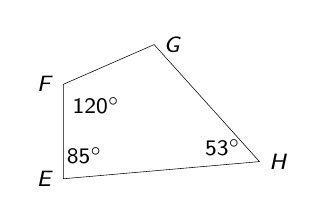
\begin{tikzpicture}
    \tkzDefPoints{0/0/E}
    \tkzDefShiftPoint[E](5:2.5){H}
    \tkzDefShiftPoint[E](90:1.2){F}
    \tkzDefShiftPoint[H](132:2){G}
    \tkzDrawPolygon(E,F,G,H)
    \tkzLabelPoints[left](E,F)
    \tkzLabelPoints[right](G,H)
    \tkzLabelAngle[pos=0.4](H,E,F){\footnotesize $85^\circ$}
    \tkzLabelAngle[pos=0.5](E,F,G){\footnotesize $120^\circ$}
    \tkzLabelAngle[pos=0.5](G,H,E){\footnotesize $53^\circ$}
    \end{tikzpicture}
\end{minipage}
\end{example}

\begin{tcolorbox}[colframe=black!20!white, opacitybacktitle=0.1, coltitle=black, title=\textbf{Equilateral Polygon}]
A polygon in which all sides are congruent.
\end{tcolorbox}

\begin{tcolorbox}[colframe=black!20!white, opacitybacktitle=0.1, coltitle=black, title=\textbf{Equiangular Polygon}]
A polygon in which all angles are congruent.
\end{tcolorbox}

\begin{tcolorbox}[colframe=black!20!white, opacitybacktitle=0.1, coltitle=black, title=\textbf{Regular Polygon}]
A polygon which is equilateral \underline{and} equiangular.
\end{tcolorbox}

\begin{tcolorbox}[colframe=black!20!white, opacitybacktitle=0.1, coltitle=black, title=\textbf{Interior Angles for a Regular Polygon}]
To find the measure of each interior angle, find the ``average" angle measure.
\[
\frac{180(n-2)}{n}
\]
\end{tcolorbox}

\begin{example}
Find the measure of each interior angle of the following.
\begin{multicols}{2}
\begin{enumerate}[(a)]
    \item A regular nonagon
    \item A regular octagon
\end{enumerate}
\end{multicols}
\end{example}

\vspace{0.5in}

\begin{tcolorbox}[colframe=black!20!white, opacitybacktitle=0.1, coltitle=black, title=\textbf{Polygon Exterior Angle Sum}]
The sum of the measures of the exterior angles of a polygon, one at each vertex, is $360^\circ$
\end{tcolorbox}
\bigskip 

Thus, to find the measure of each exterior angle of a regular polygon, divide $360^\circ$ by the number of sides. \newline 

\begin{example}
Find the measure of each exterior angle of a regular
\begin{multicols}{2}
\begin{enumerate}[(a)]
    \item Octagon
    \item Nonagon
\end{enumerate}
\end{multicols}
\end{example}

\vspace{0.5in}

\begin{example}
Find the value of $x$ in the figure below. \newline 

\begin{tikzpicture}[scale=0.8]
\tkzDefPoints{0/0/A, 2.5/0/B}
\tkzDefShiftPoint[A](125:2.25){E}
\tkzDefShiftPoint[B](70:2){C}
\tkzDefShiftPoint[A](80:4){D}
\tkzDrawPolygon(A,B,C,D,E)
\tkzDrawSegments[add = 0 and 0.75, ->, >=stealth](E,A A,B B,C C,D D,E)
\node at (A) [anchor = north west, xshift=0.25cm] {\footnotesize $14x+26$};
\node at (B) [anchor = south west, xshift=0.2cm] {\footnotesize $9x+17$};
\node at (C) [anchor = south, xshift=-0.25cm, yshift=0.6cm] {\footnotesize $8x-3$};
\node at (D) [anchor = east,xshift=-0.2cm] {\footnotesize $7x+40$};
\node at (E) [anchor = north, yshift=-1cm] {\footnotesize $12x+10$};
\draw [->, >=stealth] (-1.25,0.75) -- (-1.25,1.5);
\end{tikzpicture}
\end{example}
\end{document}
